\begin{figure} \begin{center}\centering
        \caption{Perry Birth Cohort: Total Annual Earnings, Females Age 27}
        \label{female_earn_decile1}\vspace{0.2cm}        
         \subfloat[How the Black Disadvantaged Fit into the Black Distribution at Age 27, by decile]{
                \scalebox{0.75}{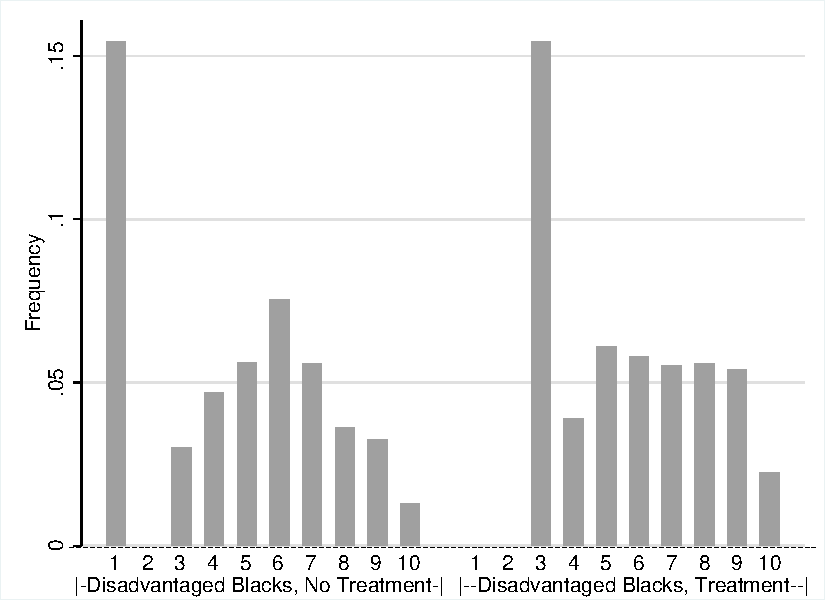
\includegraphics{female1_perry}}} \\
         \subfloat[How the Black Fit into the White Distribution at Age 27, by decile]{
                \scalebox{0.75}{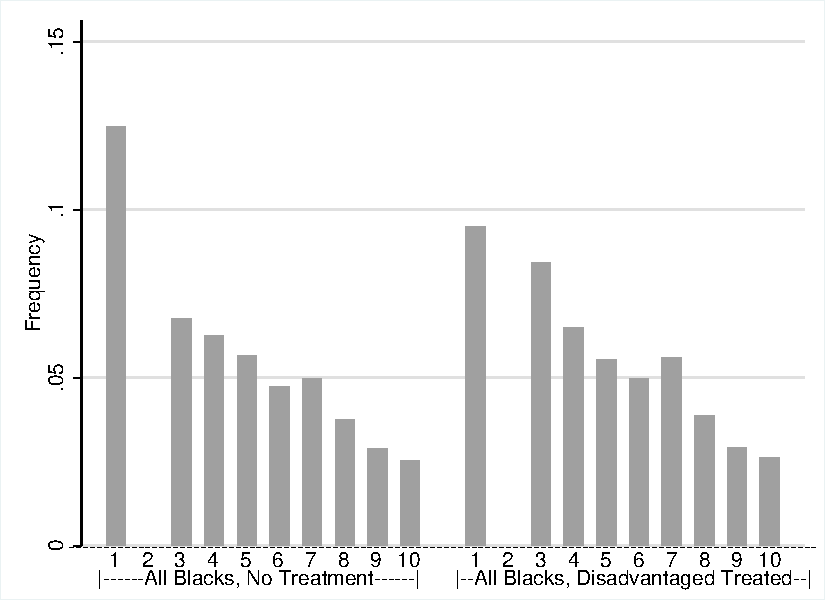
\includegraphics{female2_perry}}} \\
\end{center}
{\scriptsize {\bfseries Notes: } \raggedright The black disadvantaged group is composed of black individuals that satisfy the following criteria: 1) at least one older sibling; 2) IQ score lower than 85; 3) SES index at most 11. All the criteria are measured at age 3. The latter two criteria are approximated as in \citet{heckman2010analyzing}. The black non-disadvantaged are the individuals that violated some of the three criteria above. Black and white are representative of the cohort aged 14-22 in 1979. The left hand side plots consider the cases of the No Action Scenario (Scenario 1): the Perry Program does not influence adult outcomes. The right hand side plots consider cases of the Counter-factual Scenario (Scenario 2): we apply the gender-specific treatment effects of the Perry Program to the disadvantaged black population. We use the treatment effects calculated by \citet{heckman2010analyzing}. 
}
\end{figure}


\begin{figure} \begin{center}\centering
        \caption{Perry Birth Cohort: Total Annual Earnings, Females Age 40}
        \label{female_earn_decile2}\vspace{0.2cm}
         \subfloat[How the Black Disadvantaged Fit into the Black Distribution at Age 40, by decile]{
                \scalebox{0.75}{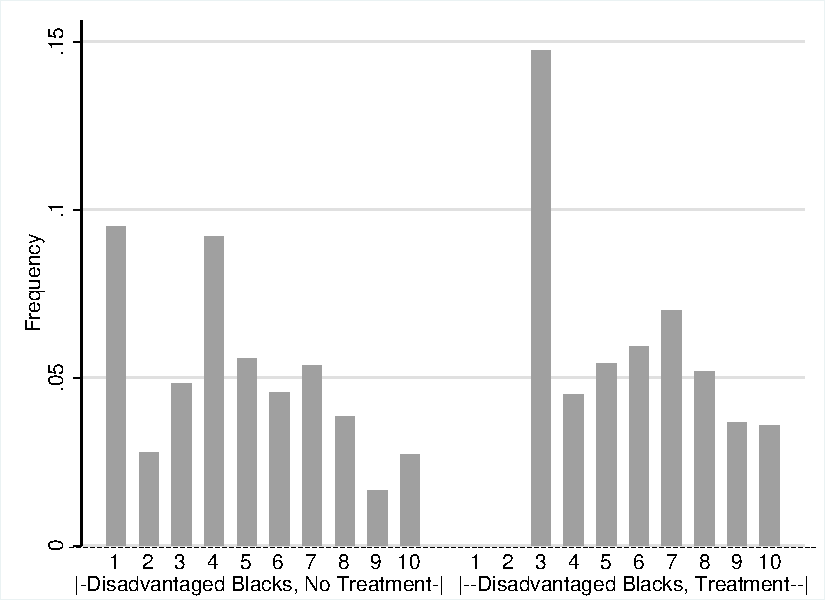
\includegraphics{female3_perry}}} \\
         \subfloat[How the Black Fit into the White Distribution at Age 40, by decile]{
                \scalebox{0.75}{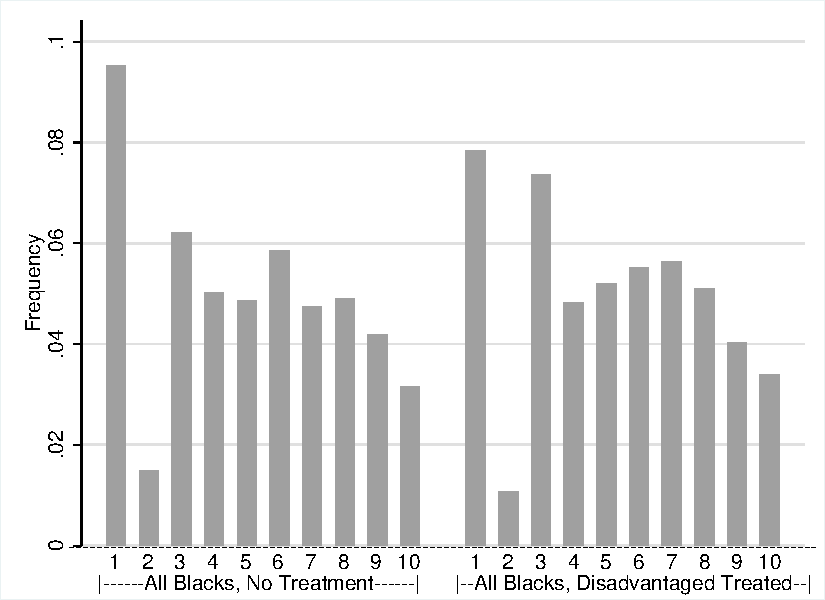
\includegraphics{female4_perry}}} \\     
\end{center}
{\scriptsize {\bfseries Notes: } \raggedright The black disadvantaged group is composed of black individuals that satisfy the following criteria: 1) at least one older sibling; 2) IQ score lower than 85; 3) SES index at most 11. All the criteria are measured at age 3. The latter two criteria are approximated as in \citet{heckman2010analyzing}. The black non-disadvantaged are the individuals that violated some of the three criteria above. Black and white are representative of the cohort aged 14-22 in 1979. The left hand side plots consider the cases of the No Action Scenario (Scenario 1): the Perry Program does not influence adult outcomes. The right hand side plots consider cases of the Counter-factual Scenario (Scenario 2): we apply the gender-specific treatment effects of the Perry Program to the disadvantaged black population. We use the treatment effects calculated by \citet{heckman2010analyzing}. 
}
\end{figure}


\begin{figure} \begin{center}\centering
        \caption{Perry Birth Cohort: Total Annual Earnings, Males Age 27}
        \label{male_earn_decile1}\vspace{0.2cm}
        
         \subfloat[How the Black Disadvantaged Fit into the Black Distribution at Age 27, by decile]{
                \scalebox{0.75}{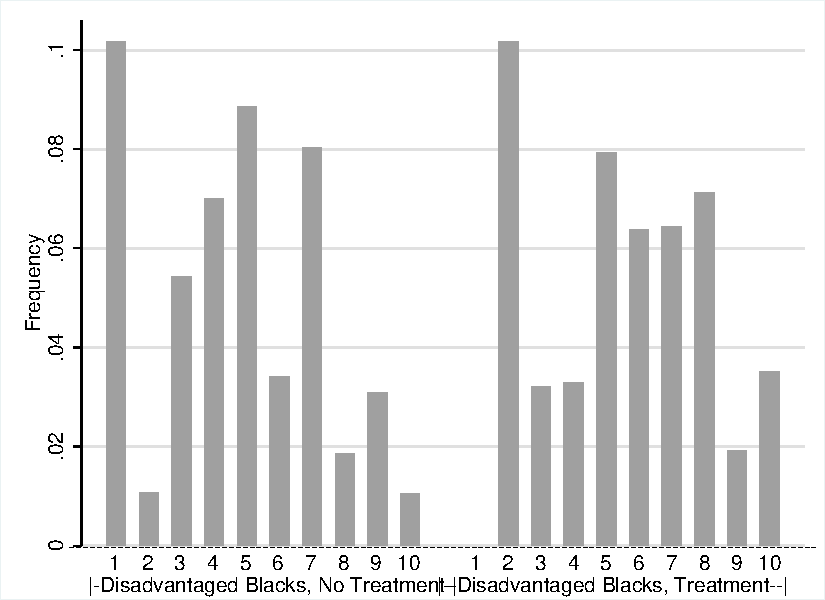
\includegraphics{male1_perry}}} \\
         \subfloat[How the Black Fit into the White Distribution at Age 27, by decile]{
                \scalebox{0.75}{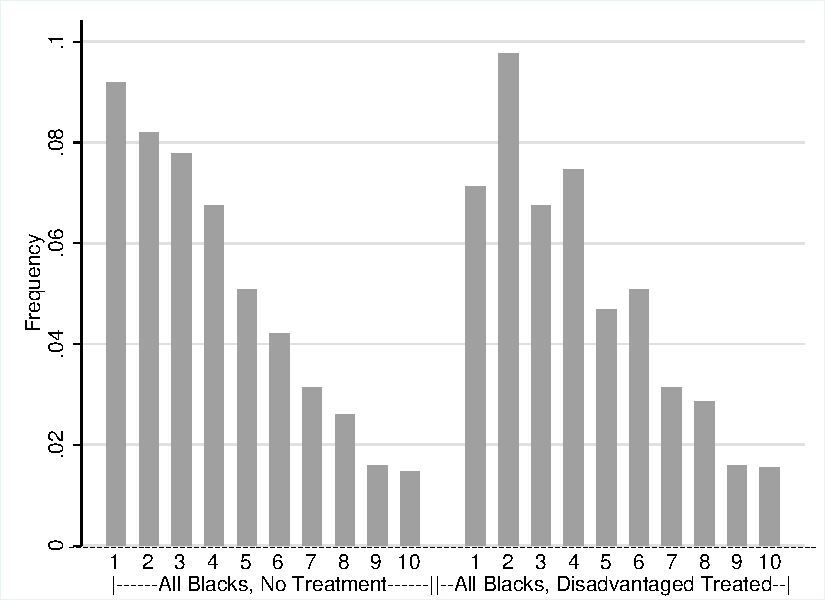
\includegraphics{male2_perry}}} \\
\end{center}
{\scriptsize {\bfseries Notes: } \raggedright The black disadvantaged group is composed of black individuals that satisfy the following criteria: 1) at least one older sibling; 2) IQ score lower than 85; 3) SES index at most 11. All the criteria are measured at age 3. The latter two criteria are approximated as in \citet{heckman2010analyzing}. The black non-disadvantaged are the individuals that violated some of the three criteria above. Black and white are representative of the cohort aged 14-22 in 1979. The left hand side plots consider the cases of the No Action Scenario (Scenario 1): the Perry Program does not influence adult outcomes. The right hand side plots consider cases of the Counter-factual Scenario (Scenario 2): we apply the gender-specific treatment effects of the Perry Program to the disadvantaged black population. We use the treatment effects calculated by \citet{heckman2010analyzing}. 
}
\end{figure}



\begin{figure} \begin{center}\centering
        \caption{Perry Birth Cohort: Total Annual Earnings, Males Age 40}
        \label{male_earn_decile2}\vspace{0.2cm}

         \subfloat[How the Black Disadvantaged Fit into the Black Distribution at Age 40, by decile]{
                \scalebox{0.75}{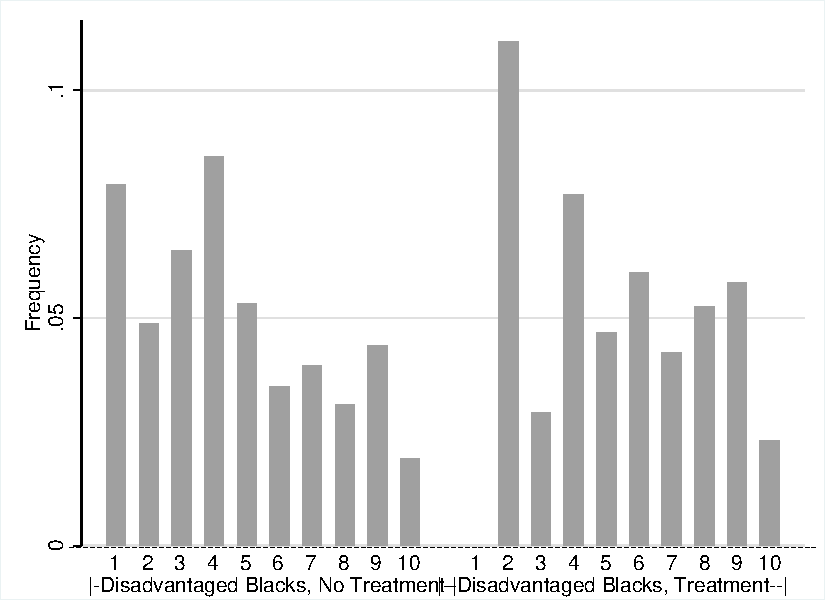
\includegraphics{male3_perry}}} \\
         \subfloat[How the Black Fit into the White Distribution at Age 40, by decile]{
                \scalebox{0.75}{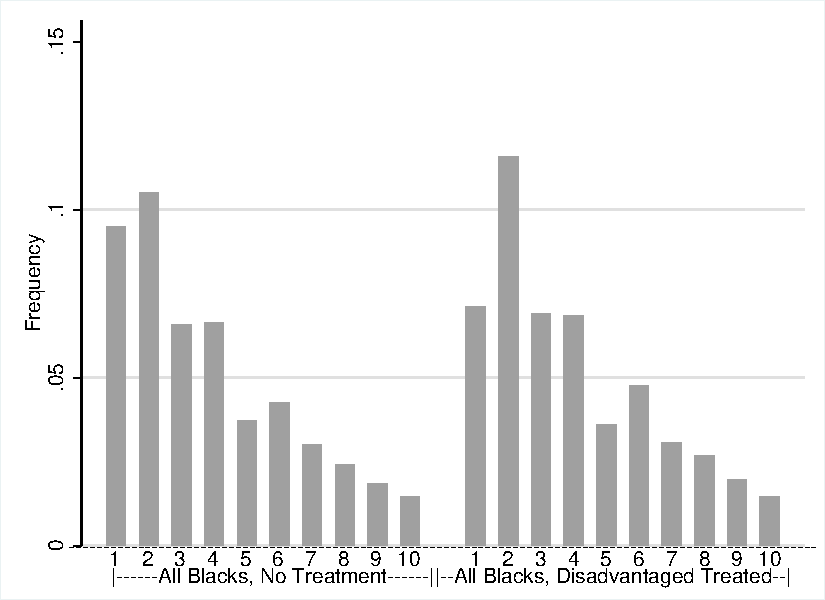
\includegraphics{male4_perry}}} \\ 
\end{center}
{\scriptsize {\bfseries Notes: } \raggedright The black disadvantaged group is composed of black individuals that satisfy the following criteria: 1) at least one older sibling; 2) IQ score lower than 85; 3) SES index at most 11. All the criteria are measured at age 3. The latter two criteria are approximated as in \citet{heckman2010analyzing}. The black non-disadvantaged are the individuals that violated some of the three criteria above. Black and white are representative of the cohort aged 14-22 in 1979. The left hand side plots consider the cases of the No Action Scenario (Scenario 1): the Perry Program does not influence adult outcomes. The right hand side plots consider cases of the Counter-factual Scenario (Scenario 2): we apply the gender-specific treatment effects of the Perry Program to the disadvantaged black population. We use the treatment effects calculated by \citet{heckman2010analyzing}. 
}
\end{figure}

